\chapter{The cobordism category}\label{CobCat}
We now get to the most important example of symmetric monoidal category in this course: the
 symmetric monoidal category of cobordisms\footnote{See chapter 14 of \cite{FreedBordism}.}. This is
 what will allow us to define a topological field theory.
\begin{notat}
   Note that, if not explicitly stated we will mean \emph{smooth} manifold when we write manifold.
\end{notat}
\begin{defn}[Bordism Category]\label{Bordism Cat Defn}
    The objects are closed $(n-1)$-dimensional manifolds. A morphism from $M$ to $N$ is a \textit{diffeomorphism class of} bordisms (to be soon defined) from $M$ (\textit{source}) to $N$ (\textit{target}), that is, a compact manifold with boundary $\Sigma$ together with embeddings
    $$\theta_0: [0,1) \times M \hookrightarrow \Sigma$$
    $$\theta_1: (-1,0] \times N \hookrightarrow \Sigma$$
    with a partition $p: \de \Sigma \to \{0,1\}$ such that
       $$\theta_0(0,M)= (\de\Sigma)_0 := p^{-1}(0)$$
       $$\theta_1(0,N)= (\de\Sigma)_1 := p^{-1}(1)$$
     Composition is given by gluing\footnote{We define bordisms with the definition with collars because it is easier to see how to glue them.} bordisms together along a common boundary: if $\Sigma$ is a morphism from $M$ to $N$ and $\Sigma'$ from $N$ to $P$ we can define $\Sigma' \circ \Sigma:=\Sigma\cup_N\Sigma'$ as (a rappresentative of) the composition morphism. 
     \begin{figure}
         \centering
         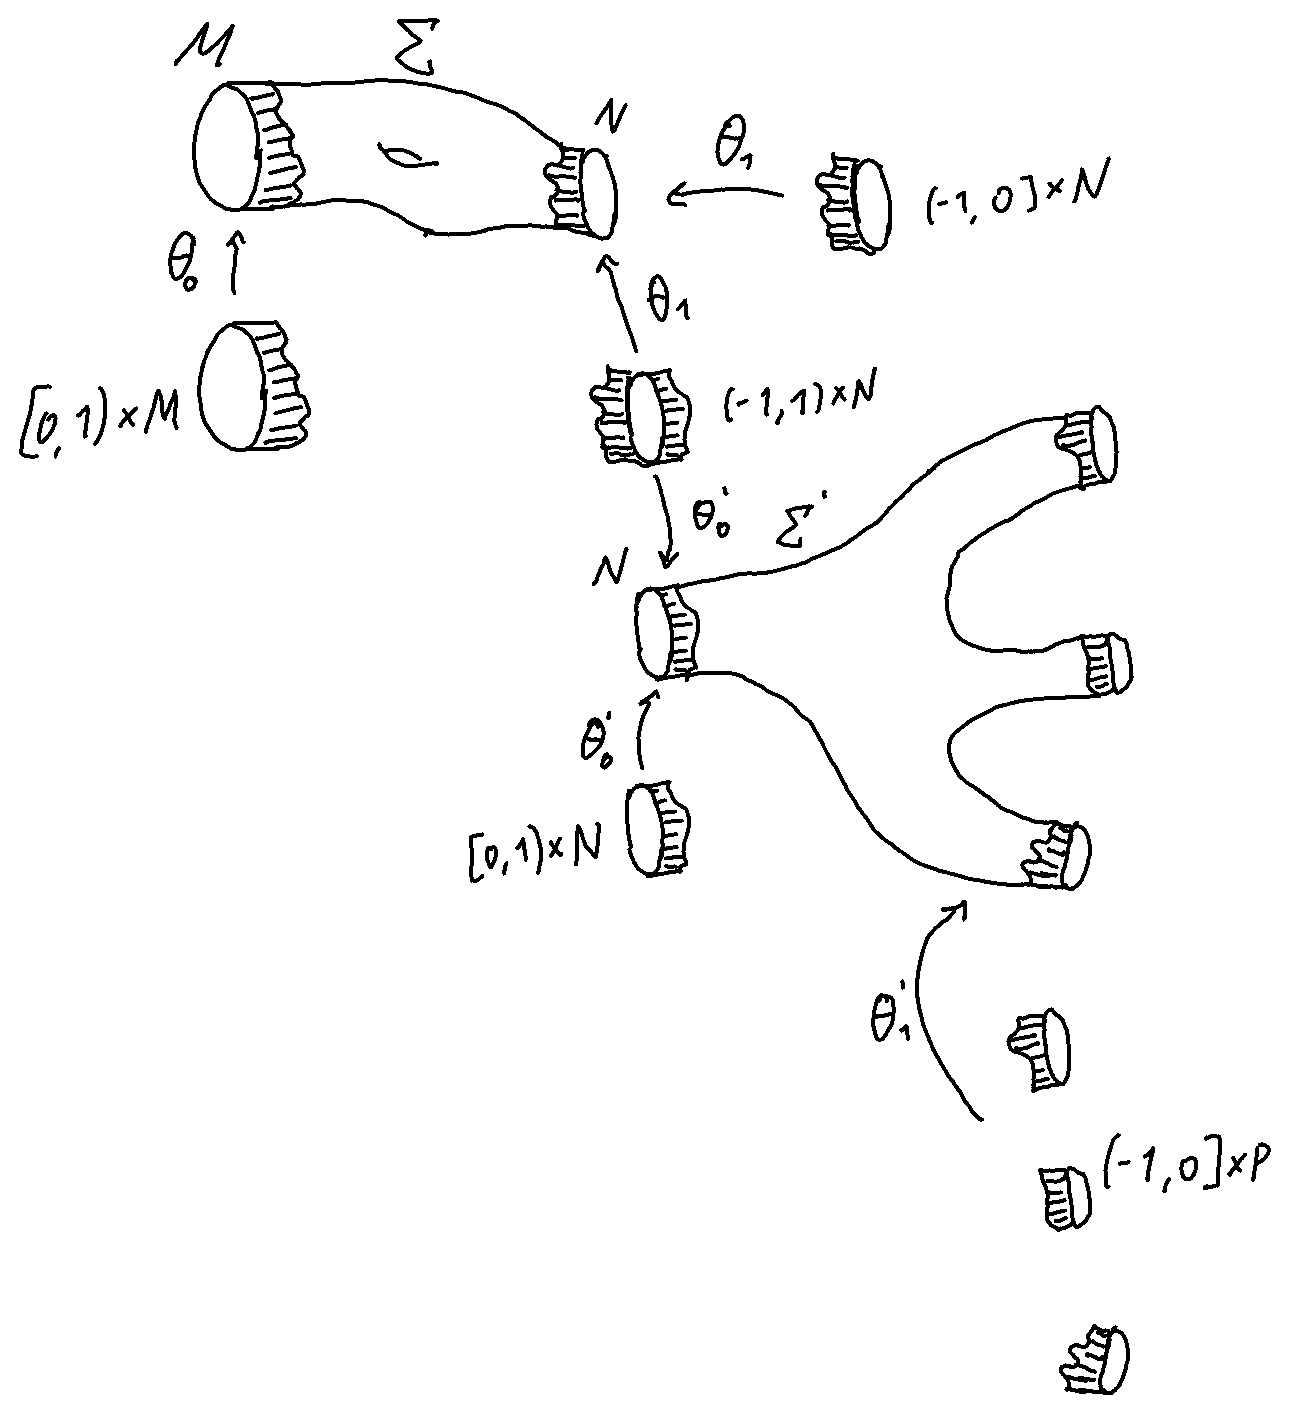
\includegraphics[width=70mm,scale=0.5]{images/Lecture 10/GlueBord.png}
         \caption{This is an illustration of gluing of two bordisms along their common boundary.}
         \label{Gluing Bordisms}
     \end{figure}
    The gluing of manifolds is associative. 

    \noindent In order for this to actually be a category there must be a identity morphisms for each object: take $M$ to be a suitable manifold, we can then take $M \times [0,1]$ to be the identity morphism. 
    However, one could also take $M \times [0,2]$ which is diffeomorphic to $M \times [0,1]$ but \textit{not} strictly identical, on the nose.

    \noindent That is why we took a \textit{diffeomorphism class} of bordisms. 
\end{defn}
\begin{notat}
    $\nCob=\Bordn$, meaning that objects are closed $(n-1)$-dimensional manifolds and morphisms are diffeomorphism classes of bordisms. Moreover, we indicate that the closed manifolds are oriented and the bordisms orientation preserving with $\Bordnor$ or equivalently $\nCob^{\orient}$.
\end{notat}
Let us explicitly state what is meant by diffeomorphism of bordisms:
\begin{defn}
    A diffeomorphism of bordisms from $M$ to $N$, $(\Sigma, p, \theta_0, \theta_1) \to (\Sigma', p', \theta_0', \theta_1')$ is a diffeomorphism $\phi: \Sigma \to \Sigma'$ of manifolds with boundary 
    % https://q.uiver.app/#q=WzAsNCxbMSwwLCJNIl0sWzAsMSwiXFxTaWdtYSJdLFsyLDEsIlxcU2lnbWEnIl0sWzEsMiwiTiJdLFswLDEsIlxcdGhldGEoMCwtKSIsMix7InN0eWxlIjp7InRhaWwiOnsibmFtZSI6Imhvb2siLCJzaWRlIjoiYm90dG9tIn19fV0sWzEsMiwiXFxwaGkiLDJdLFsxLDIsIlxcY29uZyJdLFswLDIsIlxcdGhldGEnKDAsLSkiLDAseyJzdHlsZSI6eyJ0YWlsIjp7Im5hbWUiOiJob29rIiwic2lkZSI6ImJvdHRvbSJ9fX1dLFszLDEsIlxcdGhldGEoLSwxKSIsMCx7InN0eWxlIjp7InRhaWwiOnsibmFtZSI6Imhvb2siLCJzaWRlIjoiYm90dG9tIn19fV0sWzMsMiwiXFx0aGV0YScoLSwxKSIsMix7InN0eWxlIjp7InRhaWwiOnsibmFtZSI6Imhvb2siLCJzaWRlIjoidG9wIn19fV1d
\[\begin{tikzcd}
    & M \\
    \Sigma && {\Sigma'} \\
    & N
    \arrow["{\theta(0,-)}"', hook', from=1-2, to=2-1]
    \arrow["\phi"', from=2-1, to=2-3]
    \arrow["\cong", from=2-1, to=2-3]
    \arrow["{\theta'(0,-)}", hook', from=1-2, to=2-3]
    \arrow["{\theta(-,1)}", hook', from=3-2, to=2-1]
    \arrow["{\theta'(-,1)}"', hook, from=3-2, to=2-3]
\end{tikzcd}\]
    The commutativity of the latter diagram also implies that also extra data commute accordingly, e.g. with the partitions:
    % https://q.uiver.app/#q=WzAsMyxbMCwwLCJcXGRlXFxTaWdtYSJdLFsyLDAsIlxcZGVcXFNpZ21hJyJdLFsxLDEsIlxcezAsMVxcfSJdLFswLDEsIlxccGhpfF97XFxkZVxcU2lnbWF9Il0sWzAsMiwicCIsMl0sWzEsMiwicCciXV0=
\[\begin{tikzcd}
    \de\Sigma && {\de\Sigma'} \\
    & {\{0,1\}}
    \arrow["{\phi|_{\de\Sigma}}", from=1-1, to=1-3]
    \arrow["p"', from=1-1, to=2-2]
    \arrow["{p'}", from=1-3, to=2-2]
\end{tikzcd}\]
\end{defn}

\begin{ex}
    We have that 
        $$\Hom_{\nCob} (\emptyset, \emptyset) = \text{ \{closed $n$-manifolds\}}/\text{\{diffeomorphism\}}.$$
    For $n=2$, $\Sigma = S^2$ is a composition of
    %DRAWING

    while a genus $g$ surface is the composite:
    %DRAWING 

    which is very reminiscent of what we did in Morse theory. There we were actually also learning how the
     composition of bordisms works, this is called handle decomposition.
\end{ex}
We just saw that $\Bordn$ is a category. It has importantly also a symmetric monoidal structure:
\begin{itemize}
    \item (M) The tensor product is given by the disjoint union of manifolds, $\otimes = \amalg$, both on objects ($M \otimes N:= M \amalg N$) and on morphisms ($\Sigma \otimes \Sigma':= \Sigma \amalg \Sigma'$). Disjoint union is functorial since for $\Sigma:M\to N$, $\Sigma':M'\to N'$, $\Lambda:N\to P$, $\Lambda':N'\to P'$ in $\Bordn$ it holds that:
    \begin{itemize}
        \item $(\Sigma\cup_N\Lambda)\amalg(\Sigma'\cup_{N'}\Lambda')=(\Sigma\amalg\Sigma')\cup_{N\amalg N'}(\Lambda\amalg\Lambda')$
        \item $(M\xrightarrow{M\times[0,1]}M)\amalg(M'\xrightarrow{M'\times[0,1]}M')=M\amalg M'\xrightarrow{(M\times[0,1])\amalg (M'\times[0,1])}M\amalg M'$
        %A bit confused on how to actually check functoriality for the identity morphisms, please check if this makes sense /andrea
    \end{itemize}
    \item (O) $\unit_{\Bordn} = \emptyset$ (note that $\emptyset \amalg M \neq M$, so $\Bordn$ is not a \emph{strict} symmetric monoidal category\footnote{Note that objects were \textit{not} taken up to diffeomorphism, only morphisms.}. However, there is an isomorphism in the category since they're clearly diffeomorphic, and any diffeomorphic manifolds are cobordant. So, $\emptyset \amalg M \cong M$ in $\Bordn$, as we expect the monoidal unit to behave.
    \item (A) $M_1 \amalg (M_2 \amalg M_3) \xrightarrow{\cong} (M_1 \amalg M_2) \amalg M_3$ 
    \item (B) $\beta_{M,N}: M \amalg N \xrightarrow{\cong} N \amalg M$ and $\beta^2 = id$
\end{itemize}
\begin{rem}
    Associativity and commutativity also hold up to diffeomorphism and not strictly if one defines the disjoint union as a coproduct\footnote{A coproduct is the dual notion of (cartesian) product (see \ref{CartProd}), i.e. a coproduct in $\cat$ is a product in $\cat^{op}$.}: every coproduct is unique up to isomorphism\footnote{One can prove this in a specular way in which we proved the uniqueness of the cartesian product, see \ref{UptoIsoProds}.}, the appropriate notion of isomorphism in the category of smooth manifolds is diffeomorphism and all diffeomorphic manifolds are cobordant.
\end{rem}
\section{Definition of topological field theories}
Recall that a group homomorphism $\Omega_n \to X$ with $X$ also an abelian group is a bordism invariant, which is generally quite useful and interesting. Now that we have refined our tools and have a cobordism \emph{category} instead of the cobordism \emph{group}, the bordism invariants become symmetric monoidal functors into another symmetric monoidal category since symmetric monoidal functors are the appropriate notion of homomorphism of symmetric monoidal categories.

In particular, that's how we get a topological field theory:
\begin{defn}
    A topological field theory is a symmetric monoidal functor\footnote{See \ref{SymmMonFun} for the definition of symmetric monoidal functor.} with source $\nCob$ into a symmetric monoidal category $\cat$
    $$
        \Zf: \nCob \to \cat
    $$
\end{defn}


\begin{exercise}
\hfill
    \begin{itemize}
    \item Compare this definition to other definitions of quantum field theory.
    \item Skim through Atiyah's original paper \cite{Atiyah1988}, how does this definition compare to his set of axioms?
\end{itemize}
\end{exercise} 
After skimming through \cite{Atiyah1988} one might wonder why we defined the target category of a topological field to be just a general symmetric monoidal category and not specifically $(\Vect_{k},\otimes,k)$, as Atiyah did, or at least something similar, in the end we are studying topological quantum field theories! There are probably several reasons why someone would want to do so, for example for representation theoretic ones\footnote{e.g. \cite{stroppel2022categorification}, later we will also show that one must pick categories different to $\Vect_{k}$ in order to get interesting 3dTFTs and connect them with the Jones polynomial from knot theory.}. One of the crucial ones in particular is that one of the guiding conjectures of this field, the cobordism hypothesis, is formulated and provable without mentioning specifically $\Vect_{k}$ as a target category. See \ref{RemarkOnCobHypo} for more on this conjecture\footnote{As a spoiler: the moral of the cobordism hypothesis is that "The history of the Baez-Dolan conjecture \textit{[i.e. the cobordism hypothesis]} goes most directly through quantum field theory and its adaptation to low-dimensional topology. Yet in retrospect it is a theorem about the structure of manifolds in all dimensions..." \cite{freed2012cobordism} and hence TFTs are of interest with respect to any suitable target category, not only the ones of interest from the viewpoint of physics.}
\begin{rem}
    A TFT is a functor in a similar way that a linear representation of a group\footnote{
    In fact, some regard it a kind of representation, check out for instance around minute 18:00 of \hyperlink{https://www.youtube.com/watch?v=_9FxudwLWzg}{Catharina Stroppel: The beauty of braids - from knot invariants to higher categories}; 
    or the following quote from \hyperlink{https://www.hsm.uni-bonn.de/fileadmin/hsm/pictures/TQFT_Poster_01.pdf}{a poster for a conference on TQFTs and their connections to representation theory and mathematical physics} 
    "...a TQFT is a symmetric monoidal functor from the cobordism category to some symmetric monoidal category. It can thus be seen as a representation of a fundamental geometric category on a target category and thereby organizes interesting algebraic structures, e.g. representations of mapping class groups, in terms of cobordism categories. ..."; 
    or this quote from Daniel Freed "An extended topological field theory is a representation of the bordism category..." \cite{freed2012cobordism}.} is (see \ref{Representations of Groups}). 
    We can construct the category of TFTs in an analagous way to the one we used to define the category of linear representations of a group (see \ref{Cat of representations}): by constructing a functor category where the objects are TFTs (hence particular symmetric monoidal functors) and morphisms apt natural transformations between them\footnote{See \ref{SymmMonNat} for the definition of a symmetric monoidal natural transformation.}. 
    The category of $n$-dimensional TFTs will then be $\Hom_{\SymmMonCat}(\nCob,\cat)$ (see \ref{CatSymmMonCat} for the definition of $\SymmMonCat$, the category of all symmetric monoidal categories). 
    Similarly as with groups, one can have linear and non-linear representations, although linear representations appear more frequenly. 
    Typical examples of linear target categories are $(\AbGrp,\otimes),(\Mod_R,\otimes),(\Vect_k,\otimes)$.
\end{rem}

\begin{notat}[Category of TFTs]
    The category of TFTs is the functor category 
    $$\Hom_{\SymmMonCat}(\nCob,\cat)=\Fun^\otimes(\nCob,\cat)=\TFT_n(\cat)=\operatorname{nTFT}(\cat).$$ 
    This functor category is symmetric monoidal by defining the tensor product between TFTs pointwise: for $\Zf_1,\Zf_2\in\TFT_n(\cat)$ and $M\in\nCob$ $$(\Zf_1\otimes\Zf_2)(M):=\Zf_1(M)\otimes\Zf_2(M)$$
\end{notat}
TFTs were originally defined with Vect as the target category, $\Zf: (\nCob, \amalg) \to (\Vect, \otimes) $), see \cite{Atiyah1988}. In this case we can use the notation in equation \ref{eq:rep_of_cat} and write $\TFT_n(\Vect_k) = \Rep(\Bord_{n,n-1})$.
We can infer a few things about such TFTs:
\begin{enumerate}
    \item $\Sigma$ closed $n$-manifold, we can then view it as a bordism $\emptyset \xrightarrow{\Sigma} \emptyset$ and then we can apply $Z$ and we get $Z(\emptyset) \xrightarrow{Z(\Sigma)} Z(\emptyset)$ but $Z(\emptyset) = k$, since that's the unit in $\Vect$. So $\Zf(\Sigma)$ is a linear map from $k$ to $k$, which is entirely determined by where it sends one element. We then get that $\Zf(\Sigma)(1)$ is a diffeomorphism invariant.

    In fact, the original hope was to use TFTs to find new diffeomorphism invariants.
    \item There is a ``trivial'' TFT which on objects acts as $\Zf(M) = k$ and on morphisms as $\Zf(\Sigma) = id_k$ and we write $Z = 1$.
    \item An \emph{invertible} TFT is a TFT in which $Z(M) \cong k$ and $Z(\Sigma)$ is an isomorphism. Which is very similar but in the trivial TFT we have chosen not only $Z(M) \cong k$ but specifically $Z(M) = k$.
    This is related to ``anomalies'' in physics\footnote{To precisely see how, one needs to work with \emph{extended} TFTs, a higher categorical refinement of what we are working with now. See \cite{muller2020extended}.}.
\end{enumerate}

%TODO fix and write better, as in the exercises. Or maybe remove since it's in the exercises
\begin{ex}
    Euler characteristic ($\to$ Euler theory)

    \noindent Fix $\lambda \in \C^*$. If $M\xrightarrow{\Sigma}N$, then
    \begin{equation}
        Z_\lambda (\Sigma) := \lambda^{\chi(\Sigma)-\chi(M)}, \quad Z(M)=Z(N) = \C
    \end{equation}
    Here functoriality follows from the following: if are open subsets of $\Sigma$ and $\Sigma=\text{Int}(X)\cup int(Y)$, then
    \begin{equation}
        \chi(\Sigma) = \chi(X) + \chi(Y) - \chi(X \cap Y)
    \end{equation}
\end{ex}


\begin{defn}\label{InvertibleObject}
    Let $(\cat, \otimes, \unit_\cat)$ be a monoidal category. An object $X \in \cat$ is invertible if there is a $Y \in \cat$ such that $X \otimes Y \cong \unit_\cat$.  
\end{defn}

\begin{ex}
    In $(\Vect_k, \otimes)$, $X$ is invertible iff there is a vector space $Y$ such that $X\otimes Y \cong k$.
\end{ex}

\begin{notat}
    $\cat^\times \subset \cat$ subset of invertible objects and isomorphisms. We will later see that this is the
     underlying Picard groupoid (see \ref{PicardDualizable}) %and synonymous with $(\cat^{dualizable})^{\cong}$
      %because of \ref{InvertibleDualizable}.
\end{notat}
%dim(X \otimes Y) =  dim(X)dim (Y) = dim X = 1....?
\begin{notat}
    For some symmetric monoidal category $(\cat,\otimes,\unit_\cat)$ we sometimes abreviate that the category $\cat$ is a monoidal category with tensor product $\otimes$ by writing $\cat^\otimes$. For example, $\Set^\times$, $\Set^\amalg$, $\Vect^\oplus$, $\Vect^\otimes$.
\end{notat}

We can now rigorously define what we previously called an invertible TFT: 
\begin{defn}
    An invertible TFT is an invertible object in $\Fun^\otimes(\Bordn,\cat)$. This is equivalent to the fact that $\Zf$ factors through $\cat^\times$:
 % https://q.uiver.app/#q=WzAsMyxbMCwwLCJcXEJvcmRuXlxcYW1hbGciXSxbMiwwLCJcXGNhdF5cXG90aW1lcyJdLFsxLDEsIlxcY2F0XlxcdGltZXMiXSxbMCwxLCJcXFpmIl0sWzAsMiwiXFxiYXJ7XFxaZn0iLDIseyJzdHlsZSI6eyJib2R5Ijp7Im5hbWUiOiJkYXNoZWQifX19XSxbMiwxLCIiLDIseyJzdHlsZSI6eyJ0YWlsIjp7Im5hbWUiOiJob29rIiwic2lkZSI6InRvcCJ9fX1dXQ==
\[\begin{tikzcd}
    {\Bordn^\amalg} && {\cat^\otimes} \\
    & {\cat^\times}
    \arrow["\Zf", from=1-1, to=1-3]
    \arrow["{\bar{\Zf}}"', dashed, from=1-1, to=2-2]
    \arrow[hook, from=2-2, to=1-3]
\end{tikzcd}\]
\end{defn}

\noindent Indeed if $\cat^\otimes=\Vect_k^\otimes$, invertible objects in $\Vect_k^\otimes$ are just $k$ (up to isomorphism), so an invertible TFT $Z$ must be such that for all $M\in\Bordn$, $Z(M)\otimes Z'(M)\cong k$ and so $Z(M)\cong k\cong Z'(M)$ and so is clear why they must factor through $\cat^\times$. This definition of invertible TFT is then equivalent to the one given above.
\begin{defn}[Groupoid Completion]
    Let $\cat$ be a category. A groupoid completion $(|\cat|,i)$ is a groupoid $|\cat|$ with a functor %Reminder: ask claudia hom of monoids in freed old new instead of functor
    $i:\cat\to|\cat|$ such that if $\dat$ is a groupoid and $f:\cat\to\dat$ a functor, then there is a unique map $\tilde{f}:|\cat|\to\dat$ such that the following diagram commutes 
    % https://q.uiver.app/#q=WzAsMyxbMCwwLCJcXGNhdCJdLFsyLDAsInxcXGNhdHwiXSxbMSwxLCJcXGRhdCJdLFswLDEsImkiXSxbMCwyLCJmIiwyXSxbMSwyLCJcXHRpbGRle2Z9IiwwLHsic3R5bGUiOnsiYm9keSI6eyJuYW1lIjoiZGFzaGVkIn19fV1d
\[\begin{tikzcd}[cramped]
    \cat && {|\cat|} \\
    & \dat
    \arrow["i", from=1-1, to=1-3]
    \arrow["f"', from=1-1, to=2-2]
    \arrow["{\tilde{f}}", dashed, from=1-3, to=2-2]
\end{tikzcd}\]
\end{defn}
From the universal property of the groupoid completion, there is a further factorization of an invertible field theory: 
% https://q.uiver.app/#q=WzAsNCxbMCwwLCJcXEJvcmRuXlxcYW1hbGciXSxbMiwwLCJcXGNhdF5cXG90aW1lcyJdLFsyLDEsIlxcY2F0XlxcdGltZXMiXSxbMCwxLCJ8XFxCb3Jkbl5cXGFtYWxnIl0sWzAsMSwiXFxaZiJdLFswLDIsIlxcYmFye1xcWmZ9IiwxXSxbMiwxLCIiLDIseyJzdHlsZSI6eyJ0YWlsIjp7Im5hbWUiOiJob29rIiwic2lkZSI6InRvcCJ9fX1dLFswLDMsImkiLDJdLFszLDIsIlxcdGlsZGV7XFxaZn0iLDJdXQ==
\[\begin{tikzcd}
    {\Bord^\amalg} && {\cat^\otimes} \\
    {|\Bord^\amalg}| && {\cat^\times}
    \arrow["\Zf", from=1-1, to=1-3]
    \arrow[hook, from=2-3, to=1-3]
    \arrow["i"', from=1-1, to=2-1]
    \arrow["{\tilde{\Zf}}"', from=2-1, to=2-3]
\end{tikzcd}\]
\begin{rem}
    Note that the groupoid completion of the bordism category $|\Bordn^\amalg|$ is a Picard groupoid, see \ref{PicardDualizable}.
\end{rem}